\section{Technologie}
\subsection{Wzorzec projektowy MVC (Model-View-Controller)}
Strona internetowa powstała na bazie bardzo popularnego wśród programistów wzorca projektowego MVC. Założenia wzorca Model-Widok-Kontroler przedstawionego na rysunku \ref{fig:schemat_mvc} są bardzo proste, ich składowymi są:
\begin{itemize}
\item Model- reprezentuje logikę biznesową. Tutaj znajdują się wszelkie obiekty, które służą do wykonywania zaimplementowanej funkcjonalności danej aplikacji,
\item Widok- jest warstwą prezentacji. Odpowiada za prezentację logiki biznesowej (Modelu) użytkownikowi w przystępny sposób,
\item Kontroler- obsługuje żądania użytkownika. Odebrane zadania oddelegowuje do odpowiednich modeli.
\end{itemize}
\begin{figure}[H]
	\centering
	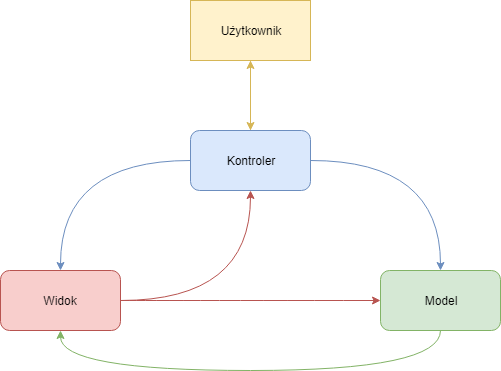
\includegraphics[scale=0.6]{mvc.png}
	\caption{Schemat klasycznego wzorca MVC}
	\label{fig:schemat_mvc}
\end{figure}

\subsection{Single Page Application}
Single Page Application (SPA) to aplikacja lub strona internetowa, która w całości wczytuje się za jednym razem. Cały potrzebny do działania strony kod (HTML, CSS, JavaScript) przesyłany jest na początku lub dodawany dynamicznie w kawałkach, zwykle w odpowiedzi na interakcje generowane przez użytkownika.
Sposób działania takiej aplikacji jest zbliżony do odczuć towarzyszących korzystaniu z aplikacji desktopowej lub mobilnej.

\subsection{Chmura obliczeniowa}
Chmura obliczeniowa jest określeniem oznaczającym model przetwarzania danych oparty na użytkowaniu usług dostarczonych przez usługodawcę. Reprezentację budowy takiego systemu przedstawiono na rysunku \ref{fig:chmura_obliczeniowa}. Użytkownik nie musi opłacać licencji, a płaci jedynie za użytkowanie danej usługi. W przypadku takich usług najpopularniejszym sposobem naliczania kosztów jest opłata od czasu użytkowania usługi.
Do najpopularniejszych udostepnianych usług należą:
\begin{itemize}
\item bazy danych,
\item maszyny wirtualne,
\item serwery,
\item hosting dla aplikacji webowych.
\end{itemize}
Przedstawicielami usługodawców udostępniających szeroki zakres usług, które zostały wykorzystane podczas tworzenia tej pracy magisterskiej jest Azure od Microsoft oraz AWS stworzony przez Amazon. Usługi obu podmiotów, które mogą być przydatne podczas tworzenia rozwiązania zostały szerzej opisane w podpunkcie \ref{azure} i \ref{aws}.
\begin{figure}[H]
	\centering
	
\includegraphics[scale=0.8]{cloud_computing.png}
	\captionsource{Obliczenia chmurowe}{http://www.justscience.in}
	\label{fig:chmura_obliczeniowa}
\end{figure}
\subsection{1-Wire} \label{1wire}
One Wire to systemowa magistrala komunikacji elektronicznej pomiędzy urządzeniami, zapewniająca przesyłanie danych oraz zasilanie urządzenia przez pojedynczy kabel. Proces ten jest możliwy dzięki stopniowemu ładowaniu kondensatora znajdującego się w odbiorniku, a następnie wykorzystanie zgromadzonej energii do zasilenia urządzenia. Do magistrali może zostać podłączonych wiele urządzeń. Każdemu z nich przydzielany jest indywidualny adres 64-bitowy. Komunikację z urządzeniami inicjuje master, w tym przypadku Raspberry Pi.
Przedstawiony protokół jest bardzo podobny do I2C, ale ze względu na wykorzystanie jedynie jednej linii danych, charakteryzuje się niższą prędkością przesyłania. Układ zazwyczaj zasilany jest napięciem o wartości 5V i służy do komunikacji pomiędzy niewielkimi urządzeniami, takimi jak np. termometr cyfrowy i mikrokontroler.

\section{Raspberry Pi} \label{raspi}
Raspberry Pi jest platformą komputerową stworzoną przez Raspberry Pi Foundation, na którą składa się pojedynczy obwód drukowany widoczny na zdjęciu \ref{fig:raspberrypi}. Pierwsza wersja tego urządzenia została zaprezentowana w 2012 roku. Na potrzeby tej pracy wykorzystano nowszą wersję urządzanie w wersji 3 B, którą została wyposażona w 4 rdzeniowy procesor i 1 GB pamięci RAM. Raspberry pozwala na podłączenie wielu urządzeń peryferyjnych za pomocą 4 portów USB lub 40 pinów GPIO. Dodatkowe złącze pozwala na podłączenie dedykowanej kamery. Dzięki znacznej ilości portów GPIO istnieje możliwość komunikacji cyfrowej z sensorami. Budowa urządzenia nie pozwala na podłączenie czujników analogowych.
\begin{figure}[H]
	\centering
	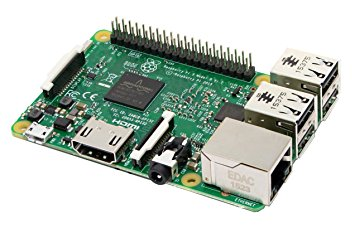
\includegraphics[scale=0.6]{raspberrypi.jpg}
	\captionsource{Raspberry Pi 3 B}{https://www.amazon.ca}
	\label{fig:raspberrypi}
\end{figure}

\subsection{Czujnik DHT 11}
\begin{figure}[H]
	\centering
	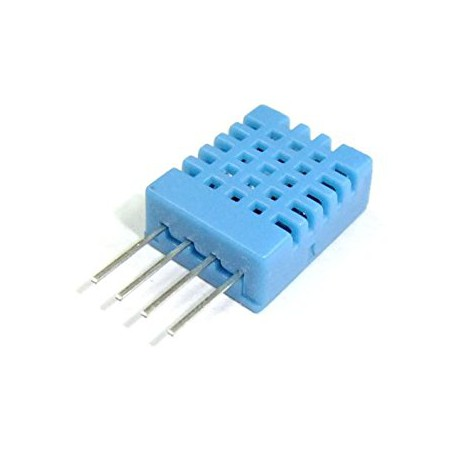
\includegraphics[scale=0.2]{dht11.jpg}
	\caption{Czujnik DHT11}
	\label{fig:dht11}
\end{figure}
Czujnik temperatury i wilgotności powietrza DHT11 jest bardzo popularnym czujnikiem z interfejsem cyfrowym. Do komunikacji wykorzystuje on protokół 1-wire opisany w rozdziale \ref{1wire}.
\begin{table}[H]
	\centering
	\caption{Parametry czujnika}
	\begin{tabular}{|c|c|}
  		\hline 
  		\bfseries Parametr & \bfseries Wartość \\
  		\hline
  		Napięcie zasilania & 3,3V do 5,5V\\
  		\hline
  		Średni pobór prądu & 0,2 mA\\
  		\hline 
  		Zakres pomiaru temperatury & od - 20\si{\degree}C do +50\si{\degree}C\\
  		\hline 
  		Zakres pomiaru wilgotności & od 5\% do 95\% wilgotności względnej\\
  		\hline 
  	\end{tabular}
\end{table}

\subsection{Raspberry Pi Camera HD}
Raspberry Pi Camera HD jest dedykowaną kamerą przeznaczoną tylko i wyłącznie do urządzenia Raspberry Pi w wersji 3, 2 oraz B+. Szybszy transfer danych niż przez port USB zapewnia dedykowane złącze minikomputera (w formie taśmy na zdjęciu \ref{fig:picamera}). Kamera posiada matrycę o rozdzielczości 8 Mpx, wspiera tryb HD 1090p, 720p oraz 640 x 480. Moduł umożliwia wykonywanie zdjęć w rozdzielczości nawet 3280 x 2464 px. Wymagane sterowniki są preinstalowane na kompatybilnych urządzeniach.
\begin{figure}[H]
	\centering
	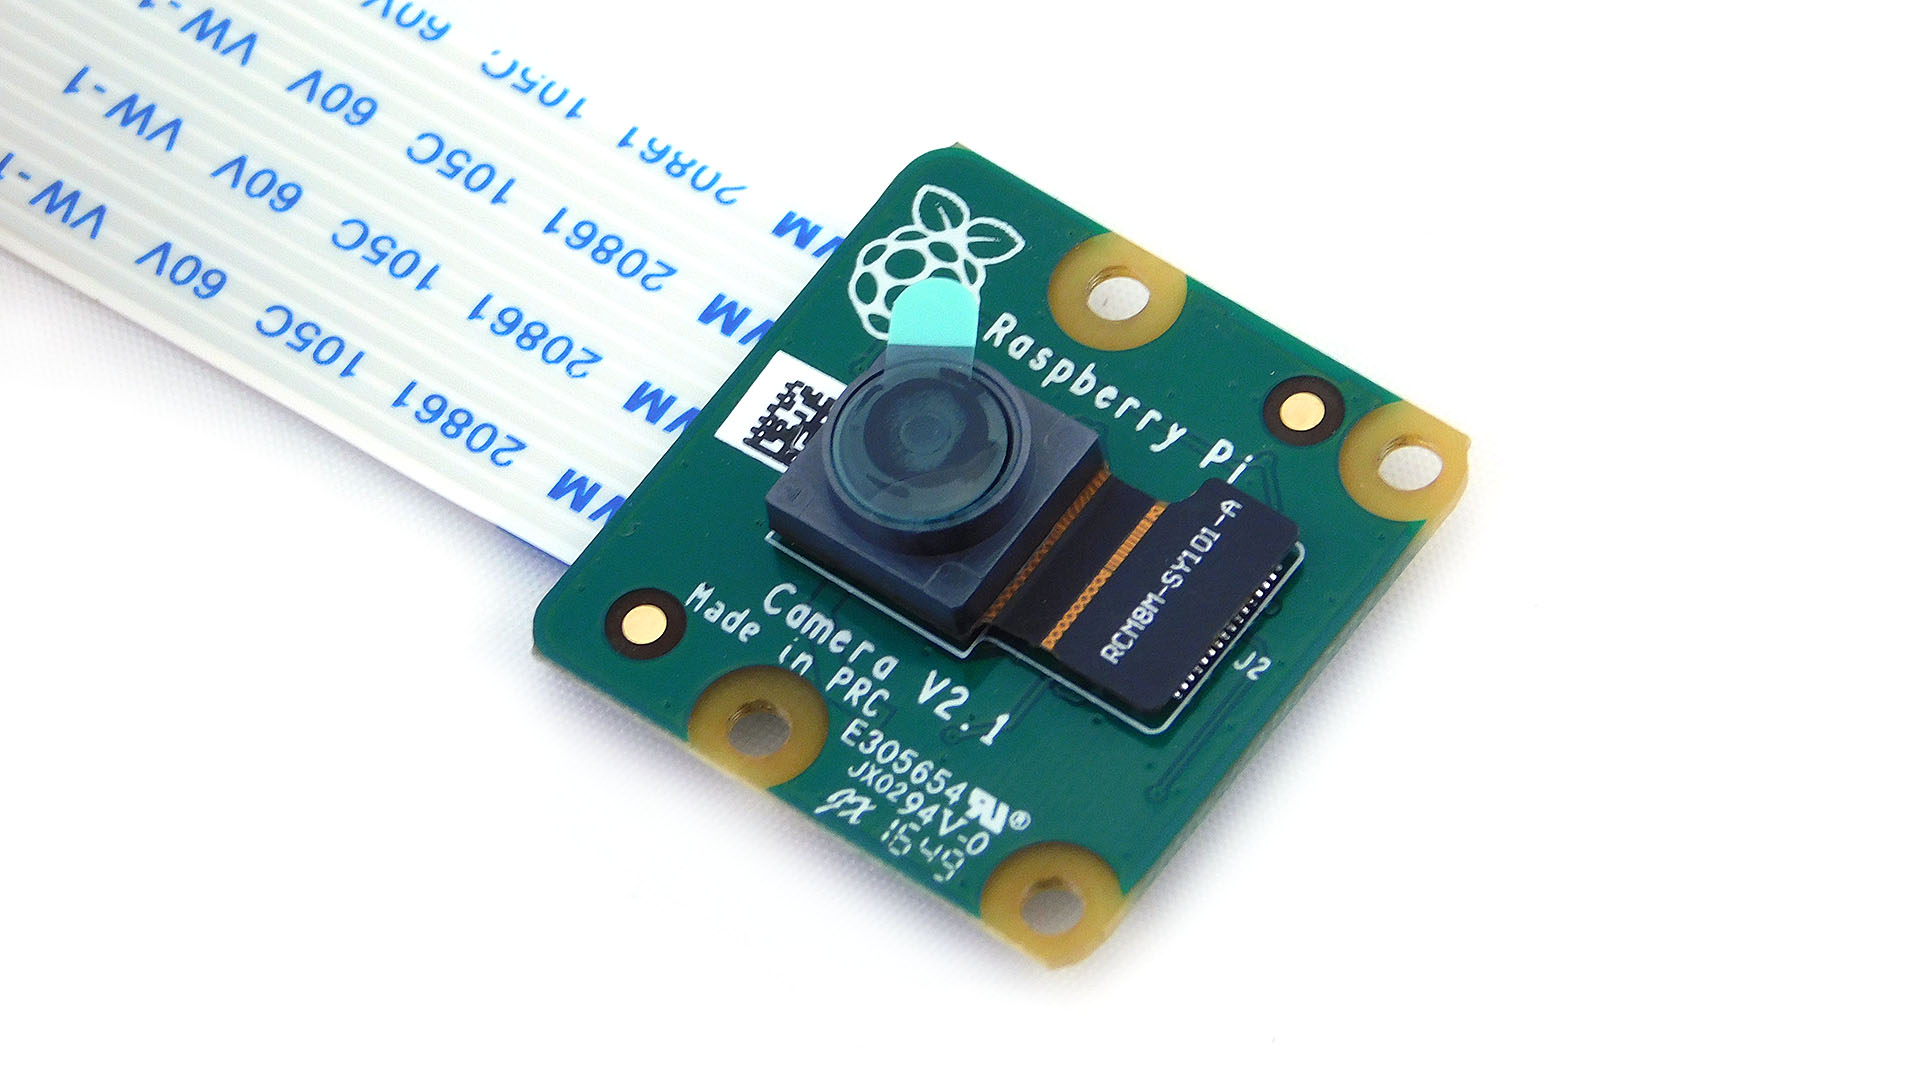
\includegraphics[scale=0.05]{picamera.jpg}
	\caption{Raspberry Pi Camera Hd}
	\label{fig:picamera}
\end{figure}

\section{Przetwarzanie obrazu}
\subsection{Thresholding}
Thresholding jest operacją polegającą na segmentacji obrazu. Segmentacja to proces podziału obrazu na części określane jako obszary, które są jednorodne pod względem pewnych wybranych własności. Podczas thresholdingu dochodzi do porównania wartości pixeli, tak by oddzielić ważne piksele od tych mniej interesujących. Przed operacją ustalana jest granica, która będzie stanowić o tym jak rozdzielone zostaną wartości.
\begin{figure}[H]
	\centering
	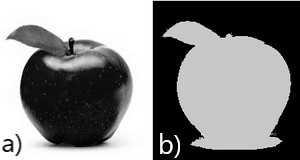
\includegraphics[scale=0.5]{efekt_thresholdingu.jpg}
	\caption{Efekt działania thresholdingu a) przed b) po}
	\label{fig:efekt_thresholdingu}
\end{figure}
Zakładając, że obraz wejściowy to $src$, wartość danego piksela oznaczono jako $src(x,y) $, a przyjętą granicę jako $thresh$. Na rysunku \ref{fig:thresholding} niebieską linią oznaczono $thresh$, a czerwonym kolorem obszar oznaczający wartość piksela. Poprzez $dst$ oznaczono obraz wyjściowy, więc $dst(x,y)$ oznacza wartość piksela o współrzednych $x,y$
\begin{figure}[H]
	\centering
	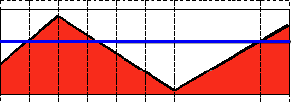
\includegraphics[scale=0.8]{thresholding.png}
	\caption{Wykres wartości obrazu $src$ przed thresholdingiem}
	\label{fig:thresholding}
\end{figure}
\begin{figure}[H]
	\centering
	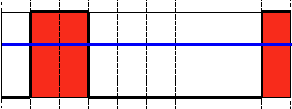
\includegraphics[scale=0.8]{thresholding_binarny.png}
	\caption{Wykres wartości pikseli obrazu $dst$}
	\label{fig:thresholding_binarny}
\end{figure}
W tej pracy zastosowano thresholding binarny konwertujący wartość każdego piksela do minimalnej lub maksymalnej. Działanie funkcji przedstawiono za pomocą poniższego wzoru.
 \begin{equation}
 \label{eq:thresholding}
 \begin{aligned}
dst(x,y) = \left\{ \begin{array}{ll}
maxValue & \textrm{gdy $src(x,y)>$thresh}\\
0 & \textrm{pozostałe}
\end{array} \right.
 \end{aligned}
\end{equation}
Porównując rysunki \ref{fig:thresholding} oraz \ref{fig:thresholding_binarny} można zaobserwować że zgodnie ze wzorem \ref{eq:thresholding} każdy piksel obrazu wejściowego poniżej wartości $thresh$ (niebieska linia), na obrazie wyjściowym ma wartość 0, a powyżej linii ma wartość maksymalną.

\subsection{Dylatacja}
Dylatacja jest operacją wykorzystywaną do przetwarzania obrazów binarnych, określaną rozszerzaniem. Proces dylatacji polega na przyłożeniu do każdego pixela na obrazie struktury o wybranym rozmiarze. Jeżeli choć jeden piksel sąsiadujący z punktem centralnym wybranej struktury ma wartość jeden to punkt centralny również otrzymuje taką samą wartość. W przeciwnym wypadku punktowi przypisywana jest wartość zero. Najkorzystniejsze efekty przynosi dylatacja strukturą przypominającą kształt koła, np 3x3 px. W efekcie dylatacji dochodzi do zwiększenia się obiektu, zniknięcia detali oraz wypełnienia pustek w niespójnym obszarze. Na rysunku \ref{fig:dylatacja} b) do obrazu przyłożono strukturę 3x3 px. W jej obszarze znaleziono jeden piksel o wartości maksymalnej(oznaczony szarym kolorem), dlatego pikselowi oznaczonemu kolorem zielonym zostaje przydzielona ta sama wartość. Przeprowadzenie operacji na całym obrazie, powoduje uzyskanie rysunku \ref{fig:dylatacja} c).
\begin{figure}[H]
	\centering
	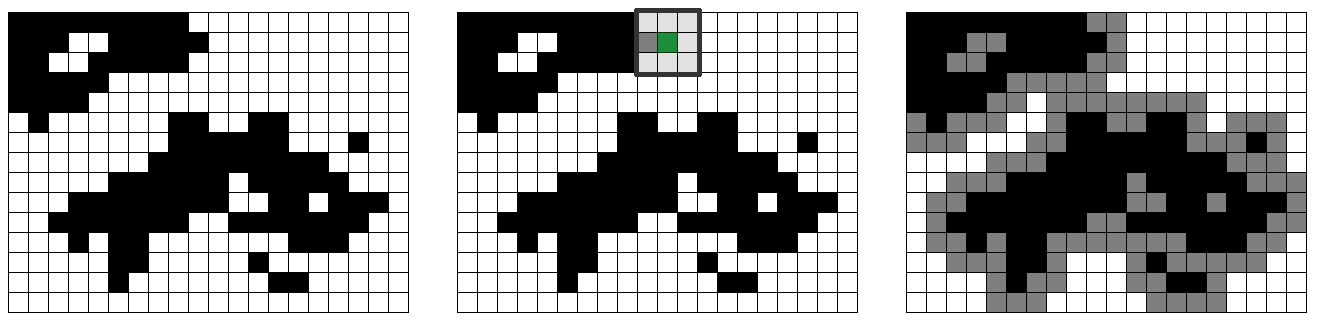
\includegraphics[scale=0.4]{dylatacja.png}
	\captionsource{Przebieg przykładowej dylatacji a) przed b) w trakcie c) po}{https://pl.wikipedia.org/wiki/Cyfrowe\_ przetwarzanie\_ obrazów\_ binarnych}
	\label{fig:dylatacja}
\end{figure}

\subsection{Rozmycie gaussowskie \textcolor{red}{DODAĆ wzór i więcej opisu}}
Rozmycie gaussowskie inaczej nazywane wygładzaniem gaussowskim to operacja przetwarzania obrazu polegająca na modyfikacji go z użyciem filtru Gaussa. Rozmycie wykorzystywane jest w celu zmniejszenia szumów oraz zakłóceń w obrazie oraz w celu zamazania detali.
\begin{figure}[H]
	\centering
	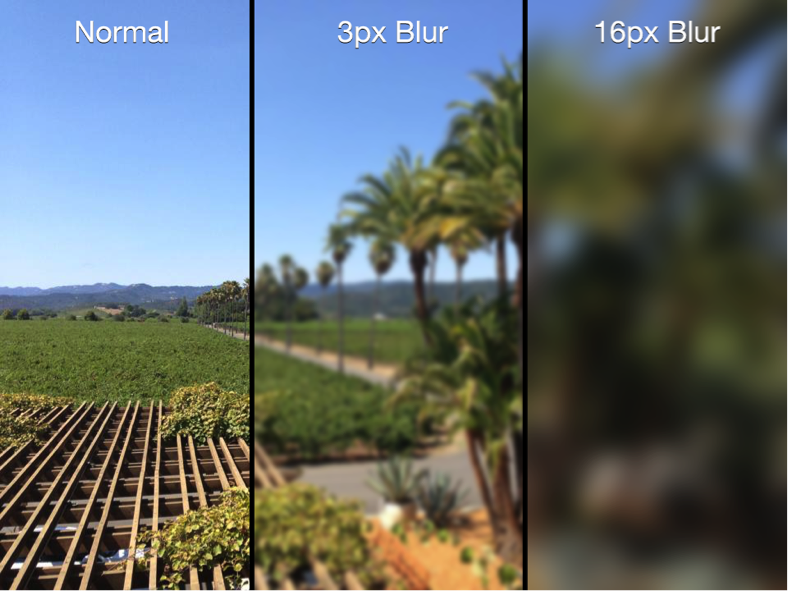
\includegraphics[scale=0.4]{rozmycie_gaussowskie.png}
	\caption{Przykład zastosowania rozmycia gaussowskiego na zdjęciu}
	\label{fig:rozmycie_gaussowskie}
\end{figure}

\subsubsection{Filtry gaussowskie}
Filtry gaussowskie należą do klasy filtrów dolnoprzepustowych, które odfiltrowują sygnały o wysokiej częstotliwości czyli np. szumy.
\cite{2}

\subsection{Klasyfikator kaskad Haar'a} \label{haar}
Detekcja obiektów klasyfikatorem kaskad Haar'a została oparta o metodę Paul'a Viola i Michael'a Jones'a– w skrócie Viola-Jones.

Algorytm Viola-Jones jest jednym z pierwszych algorytmów pozwalających na osiągnięcie zadowalających wyników w detekcji obiektów na obrazie. Został on zaproponowany w 2001 roku i został przemyślany z głównym przeznaczeniem dla detekcji twarzy. Na kluczowe koncepcje tej metody składają się:
\begin{itemize}
\item wyszukiwanie cech Haar'a,
\item integralność obrazu,
\item metoda uczenia AdaBoost (podstawowy algorytm do boostingu, metoda dzięki której z dużej liczby słabych klasyfikatorów można otrzymać jeden lepszy )
\end{itemize}

Cechy wykorzystywane w metodzie Viola-Jones opierają się na falkach Haara. Falki Haara są to sekwencje przeskalowanych kwadrato-podobnych funkcji, które razem tworzą falę(falo-podobną oscylację), podstawę z której można zbudować kwadrat. W dwóch wymiarach, fala kwadratu jest parą przylegających do siebie prostokątów, gdzie jeden jest jaśniejszy, a drugi ciemniejszy. Podstawowe szablony przedstawiono na rysunku \ref{fig:szablon_cech_haara}.
\begin{figure}[H]
	\centering
	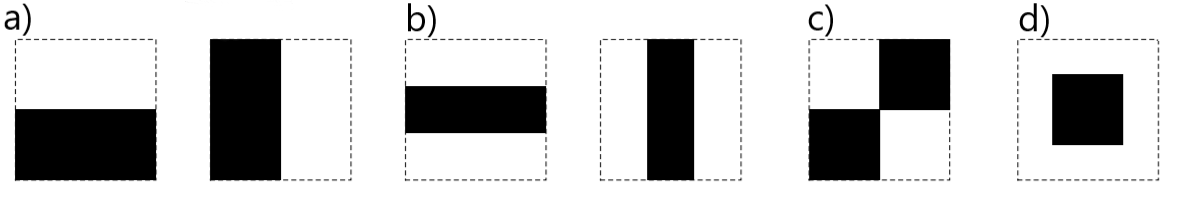
\includegraphics[scale=0.4]{szablon_cech_haara.png}
	\caption{Szablony cech Haar'a a) dwuprostokątny b) trójprostokątny c) czteroprostokątny d) centralny}
	\label{fig:szablon_cech_haara}
\end{figure}
Wartość każdej cechy jest obliczana jako różnica sumy poziomów szarości pikseli pokrywanych przez biały oraz czarny prostokąt oraz sumy poziomów szarości pikseli pokrywanych przez czarny prostokąt. Składniki tej różnicy posiadają wagi odwrotnie proporcjonalne do rozmiarów, dzięki czemu różnice wielkości dwóch obszarów są kompensowane.
\textcolor{red}{MOŻE JESZCZE WZÓR?}

\subsection{Głęboka sieć neuronowa} \label{dnn}
Pojęciem uczenia maszynowego określa się dziedzinę nauk związanych ze sztuczną inteligencją, zajmującą się badaniem algorytmów i systemów, które usprawniają swoje działanie wraz ze zdobywaniem nowej wiedzy lub też doświadczeniem. Wiedzą określamy dane uczące, które zostały wykorzystane do nauki. System może zostać usprawniony poprzez zwiększenie wiedzy systemu, które powinno pozwolić na usprawnienie procesu rozwiązywania podstawowych problemów.
\begin{figure}[H]
	\centering
	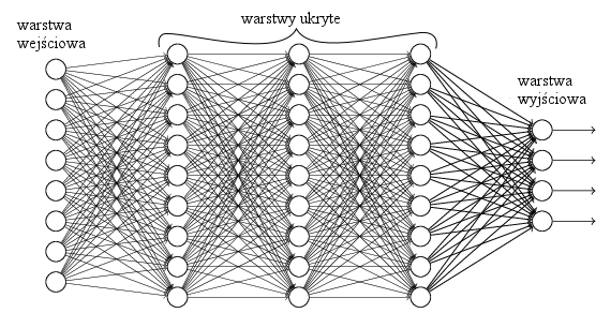
\includegraphics[scale=0.6]{schemat_dnn.png}
	\caption{Budowa głębokiej sieci neuronowej}
	\label{fig:budowa_dnn}
\end{figure}
Algorytmy głębokiego uczenia maszynowego są jednymi z najbardziej zaawansowanych. Zbudowane są one w sposób przypominający biologiczne sieci neuronowe. Głęboka sieć neuronowa składa się z neuronów rozmieszczonych na warstwach. Wiele warstw jest powodem dla którego taki rodzaj algorytmu określa się mianem głębokiego. Przykładowa budowa głębokiej sieci neuronowej została przedstawiona na rysunku \ref{fig:budowa_dnn}.

Każdy z takich “sztucznych neuronów” jest tak naprawdę informacją, która jest przesyłana dalej do następnych neuronów i ich warstw. Poszczególne warstwy “uczą” się przetwarzać kolejne cechy obiektów/obrazów/dźwięków itp., dzięki czemu są w stanie odtwarzać całe obiekty w bardzo rzeczywisty sposób. W tej pracy wykorzystano głęboką sieć neuronową do zadania wykrywania twarzy na obrazie.

\section{Azure} \label{azure}
Azure jest platformą chmurową firmy Microsoft stworzoną w modelu Paas (Platform as a Service). Platforma zbudowana jest z grupy trzech technologii zapewniających specjalizowany zestaw możliwości dla programistów, które mogą być wykorzystywane zarówno przez aplikacje uruchamiane lokalnie na komputerach użytkowników oraz aplikacje uruchamiane w chmurze. W tej pracy wykorzystano:
\begin{itemize}
    \item App Services,
    \item Azure Cognitive Services,
    \item bazy danych SQL oraz NoSQL (MSSQL, MySql, CosmicDB)
    \item maszyny wirtualne oparte o system Windows oraz kilka popularnych dystrybucji Linuxa.
\end{itemize}
\subsection{Web App Services}
Web App Services jest usługą pozwalającą na hostowanie aplikacji internetowych napisanych w jednym z wybranych języków (między innymi .Net, Node.Js, Python) bez zarządzania infrastrukturą. Do największych zalet należy automatyczna skalowalność serwisu oraz wysoka dostępność. Podczas tworzenia środowiska istnieje możliwość wyboru preferowanego systemu operacyjnego. Dużą zaletą jest możliwość wdrożenia aplikacji za pomocą jednego kliknięcia bezpośrednio z Visual Studio. Sprawne korzystanie z usługi jest możliwe dzięki szerokiemu zakresowi dokumentacji i tutoriali udostepnionych przez producenta.

\section{AWS} \label{aws}
Amazon Web Services jest platformą chmurową firmy Amazon stworzoną w modelu Paas (Platform as a Service). Jest to bardzo podobne rozwiązanie do bliźniaczego Azure. Platforma udostępnia obliczenia chmurowe na żądanie. Szeroki zakres usług dostępny jest w darmowej wersji demo, jedynym wymaganiem jest założenie konta w serwisie. Po wykorzystaniu darmowego okresu, opłaty naliczane są według zużycia danej usługi. Do podstawowych usług, które mogłyby zostać wykorzystane dla celów tej pracy należą:
\begin{itemize}
    \item Elastic Beanstalk,
    \item Rekognition,
    \item bazy danych (RDS),
    \item maszyny wirtualne (EC2).
\end{itemize}
\subsection{Elastic Beanstalk}
Elastic Beanstalk jest odpowiednikiem Azure Web App Services. Zakres dostępnych języków jest równie szeroki jak w przypadku Azure'a, ale w odróżnieniu od Microsoftu nie zawsze wspiera on najnowszych wersji produktów wymienionej firmy, a zakres możliwości konfiguracyjnych z poziomu strony internetowej jest uboższy. Podobnie jak w przypadku Azure istnieje możliwość wdrożenia aplikacji jednym kliknięciem po doinstalowaniu dedykowanego pluginu do Visual Studio.